\documentclass[tikz,border=20pt]{standalone}
\usepackage{amsmath}
\usetikzlibrary{arrows.meta, positioning, calc, angles, quotes}

\begin{document}
	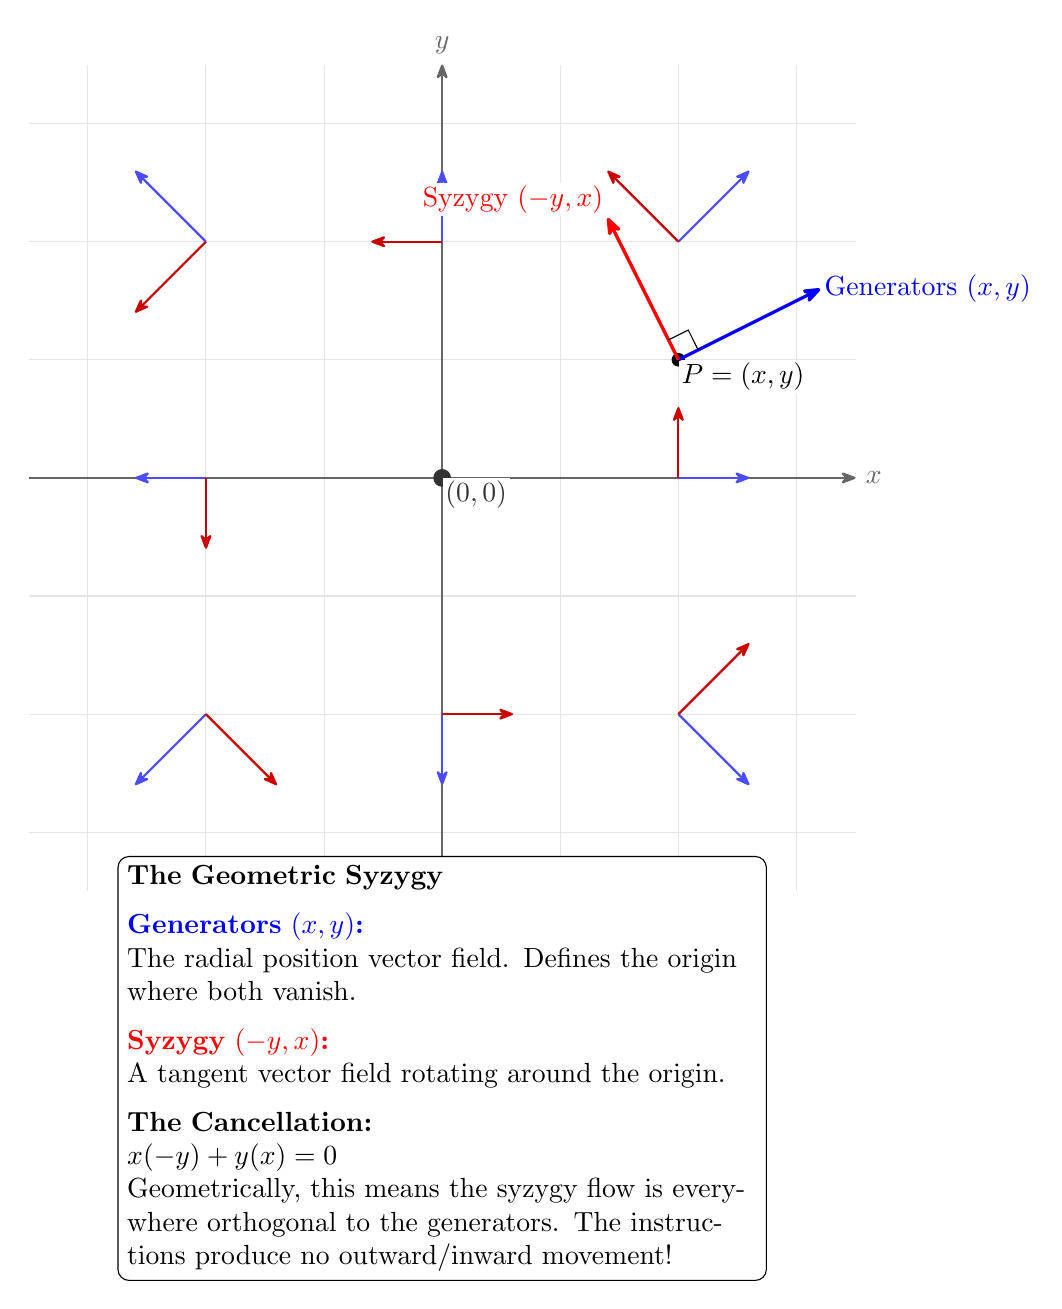
\begin{tikzpicture}[
		scale=1.5,
		radial/.style={->, >={Stealth[round]}, blue!70!white, thick},
		syzygy/.style={->, >={Stealth[round]}, red!80!black, thick},
		grid/.style={gray!20, thin},
		axis/.style={->, >={Stealth[round]}, black!60, thick}
		]
		
		% Draw grid and axes
		\draw[grid] (-3.5,-3.5) grid (3.5,3.5);
		\draw[axis] (-3.5,0) -- (3.5,0) node[right] {$x$};
		\draw[axis] (0,-3.5) -- (0,3.5) node[above] {$y$};
		
		% Draw the origin (the ideal's vanishing locus)
		% FIXED: changed bg=white to fill=white
		\filldraw[black!80] (0,0) circle (2pt) node[below right, fill=white, inner sep=1pt] {$(0,0)$};
		
		% Loop to draw the vector fields
		\foreach \x in {-2, 0, 2} {
			\foreach \y in {-2, 0, 2} {
				\ifnum \x=0
				\ifnum \y=0
				% Skip origin
				\else
				\draw[radial] (\x,\y) -- ++(0.3*\x, 0.3*\y);
				\draw[syzygy] (\x,\y) -- ++(-0.3*\y, 0.3*\x);
				\fi
				\else
				\draw[radial] (\x,\y) -- ++(0.3*\x, 0.3*\y);
				\draw[syzygy] (\x,\y) -- ++(-0.3*\y, 0.3*\x);
				\fi
			}
		}
		
		% Highlight a specific point to show the orthogonality (the cancellation)
		\coordinate (P) at (2,1);
		\coordinate (R) at ($(P) + (1.2, 0.6)$); % Scale up radial for visibility
		\coordinate (S) at ($(P) + (-0.6, 1.2)$); % Scale up syzygy for visibility
		
		\filldraw[black] (P) circle (1.5pt) node[below right, fill=white, inner sep=1pt] {$P = (x,y)$};
		\draw[->, >={Stealth[round]}, blue, line width=1.2pt] (P) -- (R) node[right, fill=white, inner sep=1pt] {Generators $(x,y)$};
		\draw[->, >={Stealth[round]}, red, line width=1.2pt] (P) -- (S) node[above left, fill=white, inner sep=1pt] {Syzygy $(-y,x)$};
		
		% Right angle marker to show cancellation
		\pic [draw, angle radius=8pt] {right angle = R--P--S};
		
		% Explanatory Text Box - Moved to the bottom so it doesn't overlap the math
		\node[draw, rounded corners, fill=white, align=left, text width=8cm] at (0,-5) {
			\textbf{The Geometric Syzygy} \\[0.2cm]
			\textcolor{blue}{\textbf{Generators $(x,y)$:}}\\
			The radial position vector field. Defines the origin where both vanish. \\[0.2cm]
			\textcolor{red}{\textbf{Syzygy $(-y,x)$:}}\\
			A tangent vector field rotating around the origin. \\[0.2cm]
			\textbf{The Cancellation:}\\
			$x(-y) + y(x) = 0$ \\
			Geometrically, this means the syzygy flow is everywhere orthogonal to the generators. The instructions produce no outward/inward movement!
		};
		
	\end{tikzpicture}
\end{document}